\chapter{Implementation}
In this chapter, we will be discussing the implementation of hardware and software of the camera that would be used for subsequent experiments.
The main specifications of the chosen cameras are shown in Table \ref{tbl:camera_specs}. These specifications are taken from the sensor data sheet and the camera manual provided by the vendors of the camera\cite{OV2640Arducam}\cite{OV5642Arducam}\cite{OV2640DS}\cite{OV5642DS}.  
\begin{table}[]
\centering
\caption{ Key Specifications Specifications of sensors Chosen}
\label{tbl:camera_specs}
\begin{tabular}{|c|c|c|}
\hline
Specification & OV2640 &  OV5642 \\
\hline
Voltage Level & 3.3/5V &  3.3/5V\\
 \hline
Frame Buffer Size & 384 KB & 8MB \\
 \hline
 Active Pixel Array Size& 1600$\times$1200&  2592$\times$1944 \\
 \hline  
 Camera Dimensions & 34mm $\times$ 24mm & 34mm $\times$24mm\\
 \hline
 Sensor Dimensions & 5725 $\mu$m $\times$ 6285 $\mu$m& 6945 $\mu$m $\times$ 6695 $\mu$m\\
 \hline
 Pixel Size & 2.2 $\mu$m $\times$ 2.2 $\mu$m & 1.4$\mu$m $\times$ 1.4 $\mu$m\\
 \hline
 Weight & 20 grams & 20 grams \\
 \hline
 \makecell{Operating \\Temperatures} & -10$\degree$C to 55$\degree$C & -10$\degree$C to 55$\degree$C \\
 \hline
 \makecell{Electronic Interfaces\\ Needed} & SPI, I2C & SPI, I2C\\
 \hline
 Dynamic Range & 50 dB & 68 dB \\
 \hline
\end{tabular}
\end{table}
\section{Embedded Software of Camera}
One of the main reasons behind choosing the OV2640 and OV5642 CMOS sensors is that they already have a ready electronic interface that can be used to interface with standard 8-bit/16-bit microcontrollers. Arducam is an open source camera that comes along with open-source hardware and software that is needed to capture images using the CMOS sensor. Arducam is a platform that provides the hardware and software components necessary to interface OV2640 and OV5642 sensors with the conventional microcontroller platforms such as Arduino. One of the core components in every camera made by Arducam is that there is a component called Arduchip\cite{Arduchip}. It is a basically an Altera MAXII CPLD EPM240 processor that facilitates DMA memory transfer between the camera memory module and components such as microcontroller and thereby helping to reduce the development time for special applications such as space where the only computational resource that would be available are low power computing platforms such as microcontrollers with only synchronous serial interfaces such as I2C, SPI, etc. 

However, using the camera comes with its own advantages and disadvantages. The main advantage of using this platform is that the platform has open-source libraries that could be used to interface with Arduino which contains ATMEGA328P, an 8-bit microcontroller. In space missions, it would not be possible to send high-powered microprocessors, and a microcontroller is used as the processing platform for various subsystems. Arducam has standard software libraries that can be used to interface with Arduino making the cumbersome and lengthy job of writing an interface software to a CMOS sensor way more easier.  A disadvantage of the hardware module is the onboard memory that it has to capture an image. The OV2640 Arducam mini camera module can capture up to $1600 \times 1200$ resolution images with or without any form of compression. However, due to the limitation of the onboard OV2640 FIFO memory AL422B, it would be possible to capture only compressed images and not full resolution RAW images. The AL422B on-board FIFO has only 384KB of memory and that is not enough to obtain a full-resolution RAW image. One of the other disadvantages is that custom code needs to be written to obtain various controls that we need for our camera. We have to write our own camera control software if we need to control factors such as exposure time, ISO, etc. as the default software uses automatic exposure control to enhance the image quality. The camera module architecture is shown in Figure \ref{fig:arducam_arch}. The OV5642 offers a greater flexibility in terms of memory as it has a larger FIFO Buffer(8 MB). Arducam has also provided APIs that can control the exposure of OV5642.

 \begin{figure}[!htbp]
\centering
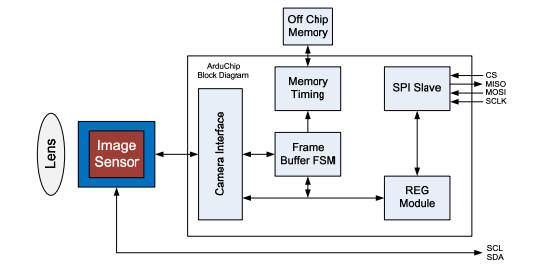
\includegraphics[width = \textwidth]{pics/arducam_architecture}
\caption{Camera Architecture of Arducam Mini OV2640 Camera Module\cite{OV5642Arducam}}
\label{fig:arducam_arch}
\end{figure}

The system for experiments is as shown in Figure \ref{fig:imp_setup}. The Arduino is connected to the sensor directly through an I2C interface. Using the I2C interface it possible to set registers that control the functioning of the camera such as the output format, digital signal processing, etc. SPI interface is used to transfer the image data from the camera module to the Arduino. The Arduino upon receiving the image data either writes it to an  SD card or sends it to the software on the PC through the USB connection. The software flow is shown in Figure \ref{fig:arducam_software}. We use the same software flow for both the CMOS sensors as the APIs are designed for use with many sensor models. The same set of libraries can be used for different CMOS sensors by simply adding some preprocessor directives to a \texttt{memorysaver.h} header file provided in the open-source library. To see the images on the PC, the vendor has provided a host PC software(not open source) and firmware which uses USB-UART to transfer images from the Arduino to PC. The firmware could be modified to ignore certain commands coming from the PC and using this we were able to modify the camera settings to our advantage. 
\begin{figure}[!htbp]
\centering
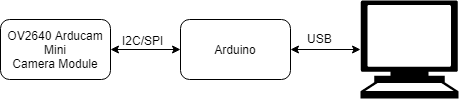
\includegraphics[scale=0.75]{pics/implementation_setup}
\caption{Implementation Setup}
\label{fig:imp_setup}
\end{figure}

One of the important factors that need to be controlled in camera is the exposure time. The Arducam libraries provide APIs for 10 different exposure levels for the OV5642 sensor. However, no such APIs are available for OV2640. Since OV2640 consumes lower power, it was decided to start the experiments with this camera. So, we need to write custom software to control the exposure level of this camera. The Arducam APIs used for the software are shown in Table \ref{fig:arducam_software}. The details of more APIs can be found in the software application notes\cite{ArducamSoftwareApp}. The default camera settings were used with only modifications to exposure in the case of OV2640 module. The CMOS sensor can be directly accessed using \texttt{wrSensorReg16\_8, wrSensorReg8\_8} functions which provide I2C bus access to the CMOS sensor.
\begin{figure}[!htbp]
\centering
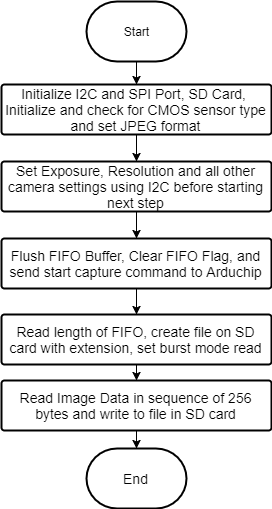
\includegraphics[scale  = 0.5]{pics/SoftwareFlowOV2640}
\caption{Software Flow used for image acquisition from CMOS sensors}
\label{fig:arducam_software}
\end{figure}


\begin{table}[!ht]
\centering
\caption{ Details of Main APIs used}
\label{tbl:camera_apis}
\begin{tabular}{|c|c|c|}
\hline
API & Function \\
\hline
\texttt{InitCAM} & Initialize Camera Module\\
\hline
\texttt{set\_format} & \makecell{JPEG an BMP output formats \\can be selected}\\
\hline

\makecell{\texttt{clear\_fifo\_flag}\\ \texttt{read\_fifo\_length}\\
\texttt{set\_fifo\_burst} \\
\texttt{flush\_fifo}} & \makecell{These functions are \\used to control the FIFO buffer, \\read the size of \\the image  and \\to reset them when needed}  \\

\hline
\texttt{write\_reg} & \makecell{This function is used to write \\values to the specified register\\ address on the Arduchip.}\\
\hline
\texttt{\makecell{wrSensorReg16\_8\\wrSensorReg8\_8}} & \makecell{These functions are used to\\ set camera \\ registers using I2C. The first function \\ is used for 16-bit register\\ addresses and the \\second function is used for\\ 8-bit addresses}  \\
\hline
\texttt{\makecell{OV2640\_set\_JPEG\_size\\ \texttt{OV5642\_set\_JPEG\_size}}} & \makecell{These functions are used \\to set the resolution of the\\ output image } \\
\hline
\texttt{OV5642\_set\_Exposure\_level} & \makecell{This functions are used \\to set the exposure level of the \\OV5642 CMOS sensor}\\
\hline
\end{tabular}
\end{table}
\subsection{Exposure Control of OV2640}
In order to do experiments, it was required to control the exposure of the camera. In the default driver that was provided by the vendor, the exposure was automatically set using the Automatic Exposure Control (AEC) feature in the sensor. So, a modification was needed in the driver software. Fortunately, the driver is open source and there were libraries that could assist in setting the onboard registers through the I2C interface on the Arduino. First, let us have a look at how exposure control works in an OV2640 camera. All rolling shutter image sensors including OV2640 expose the sensor one-line at a time i.e. pixels in the same line are exposed at the same time and different pixels in different lines are exposed at a different time. 

\begin{figure}[!ht]
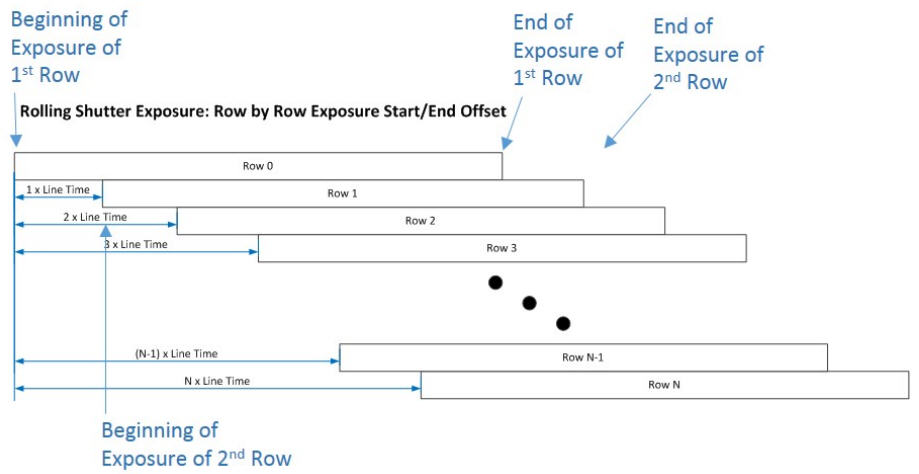
\includegraphics[width=\textwidth]{pics/rolling_shutter}
\caption{Rolling Shutter Operation on OV2640\cite{RollingShutterOV2640}}
\label{fig:RollingShutterOV2640}
\end{figure}

\begin{figure}[!ht]
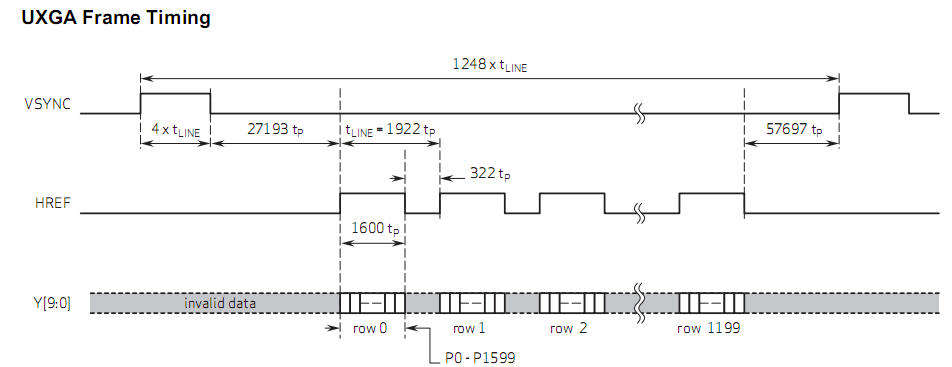
\includegraphics[width=\textwidth]{pics/OV2640timing}
\caption{Shutter Timing Diagram of OV2640\cite{RollingShutterOV2640}}
\label{fig:ShutterTimingOV2640}
\end{figure}


So, the minimum exposure time would be one line time and the maximum exposure time would be the frame time. This is illustrated in Figure \ref{fig:RollingShutterOV2640}. By default, the pixel clock is set at 36MHz. We can calculate the minimum line time using the following equation:

$$
Minimum\ Exposure\ Time = \frac{1}{Pixel\ Clock} * Pixel \ Clockes \ per \ line 
$$
As shown in Figure \ref{fig:ShutterTimingOV2640}, one line consists of 1922 pixel clocks(1600 for pixel data and 322 clocks of horizontal blanking). So the minimum exposure time would be 53.39$\mu$seconds and the maximum exposure time would be the frame time(multiply line time by 1200 + 44 lines of vertical blanking) which would be 66.63ms\cite{RollingShutterOV2640}. In order to control the exposure of the camera, it is necessary to modify registers of address 4, 10, 13, 45(See Figure \ref{fig:OV2640Registers}). So, these registers were modified according to the required exposure time value. The driver software on the Arduino was modified to obtain different exposure times. The images of a laser beam captured(with lens) with different exposure times using the software developed are shown in Figure \ref{fig:exptests}.

\begin{figure}[!ht]
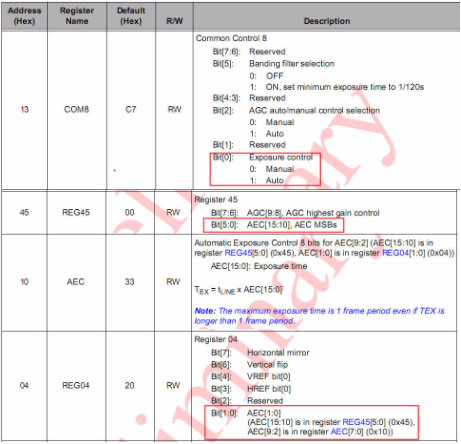
\includegraphics[width=\textwidth]{pics/exposure/OV2640ExposureRegisters}
\caption{Registers to be changed to control exposure of OV2640\cite{OV2640DS}\cite{RollingShutterOV2640}}
\label{fig:OV2640Registers}
\end{figure}


    \begin{figure}[ht]
    \centering
    \begin{subfigure}{0.5\textwidth}
    \centering
        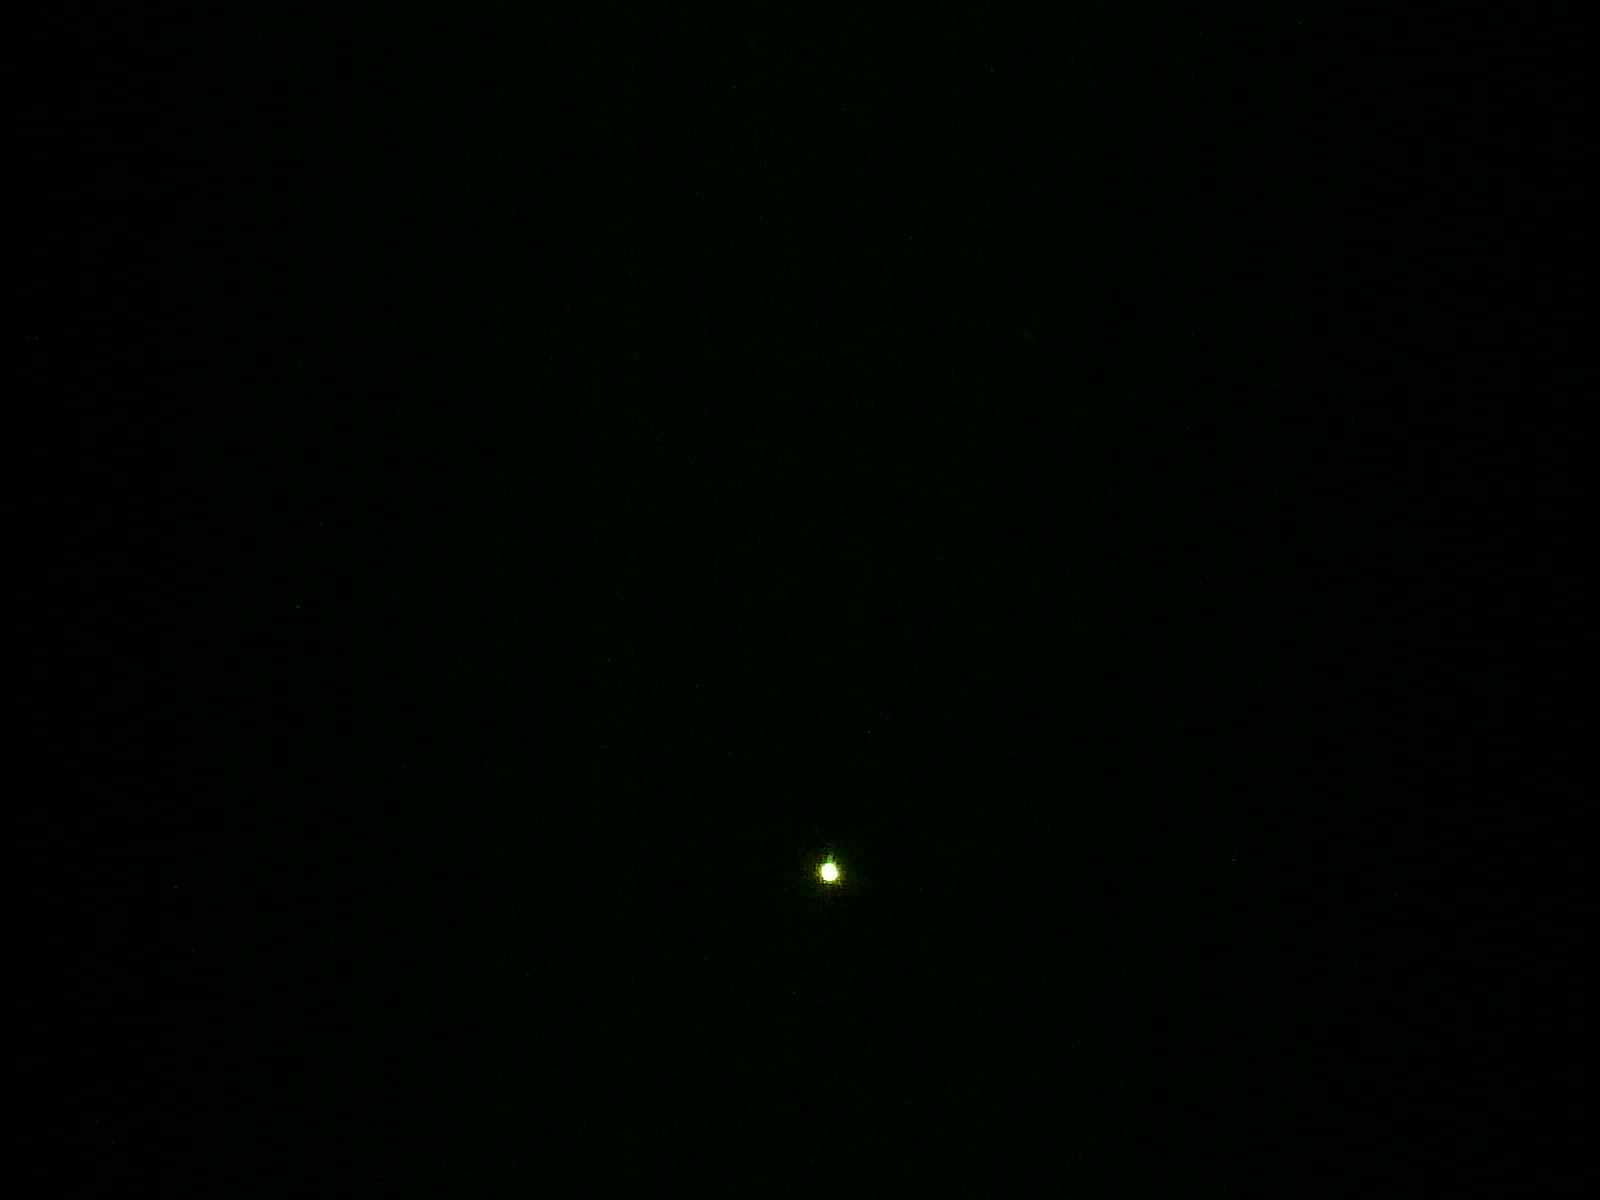
\includegraphics[width=0.5\linewidth]{pics/exposure/60us}
        \caption{60 $\mu$seconds}
        \label{fig:exp60us}
    \end{subfigure}%
    \begin{subfigure}{0.5\textwidth}
    \centering
        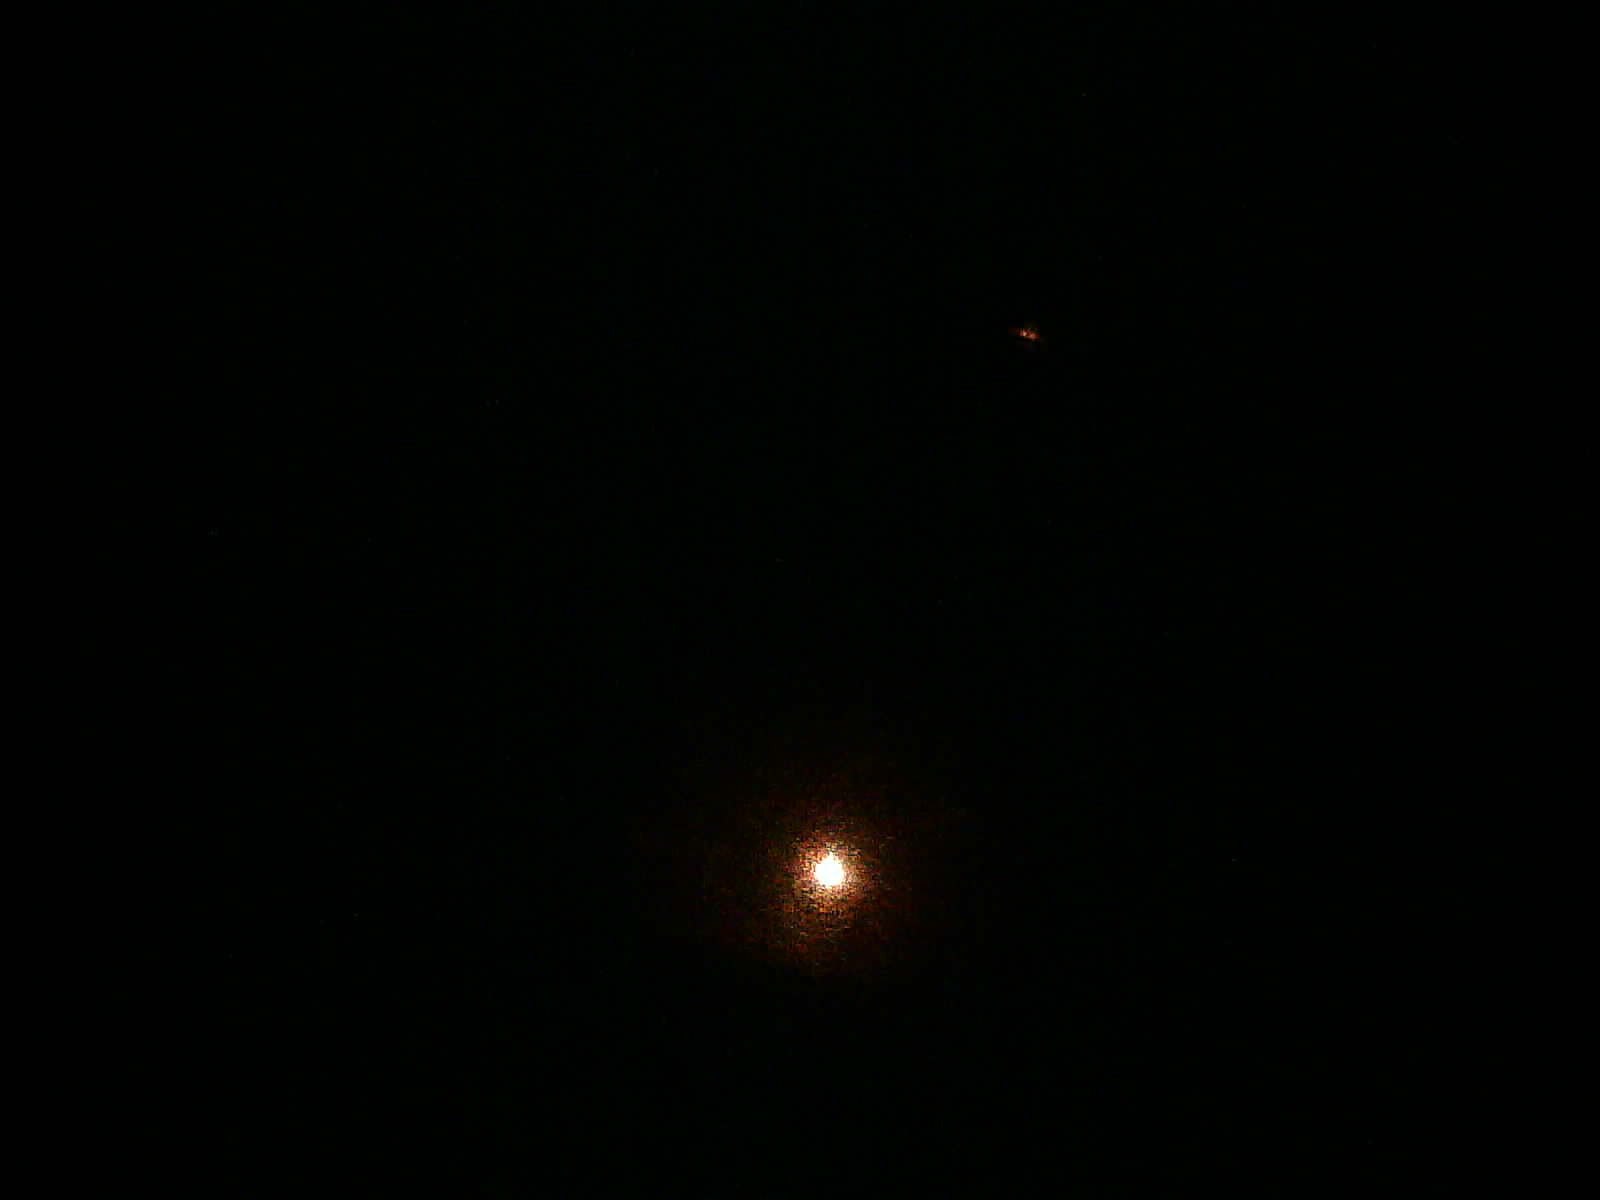
\includegraphics[width=0.5\linewidth]{pics/exposure/1ms}
        \caption{1ms}
        \label{fig:exp1ms}
    \end{subfigure}
    
    \begin{subfigure}{0.5\textwidth}
    \centering
        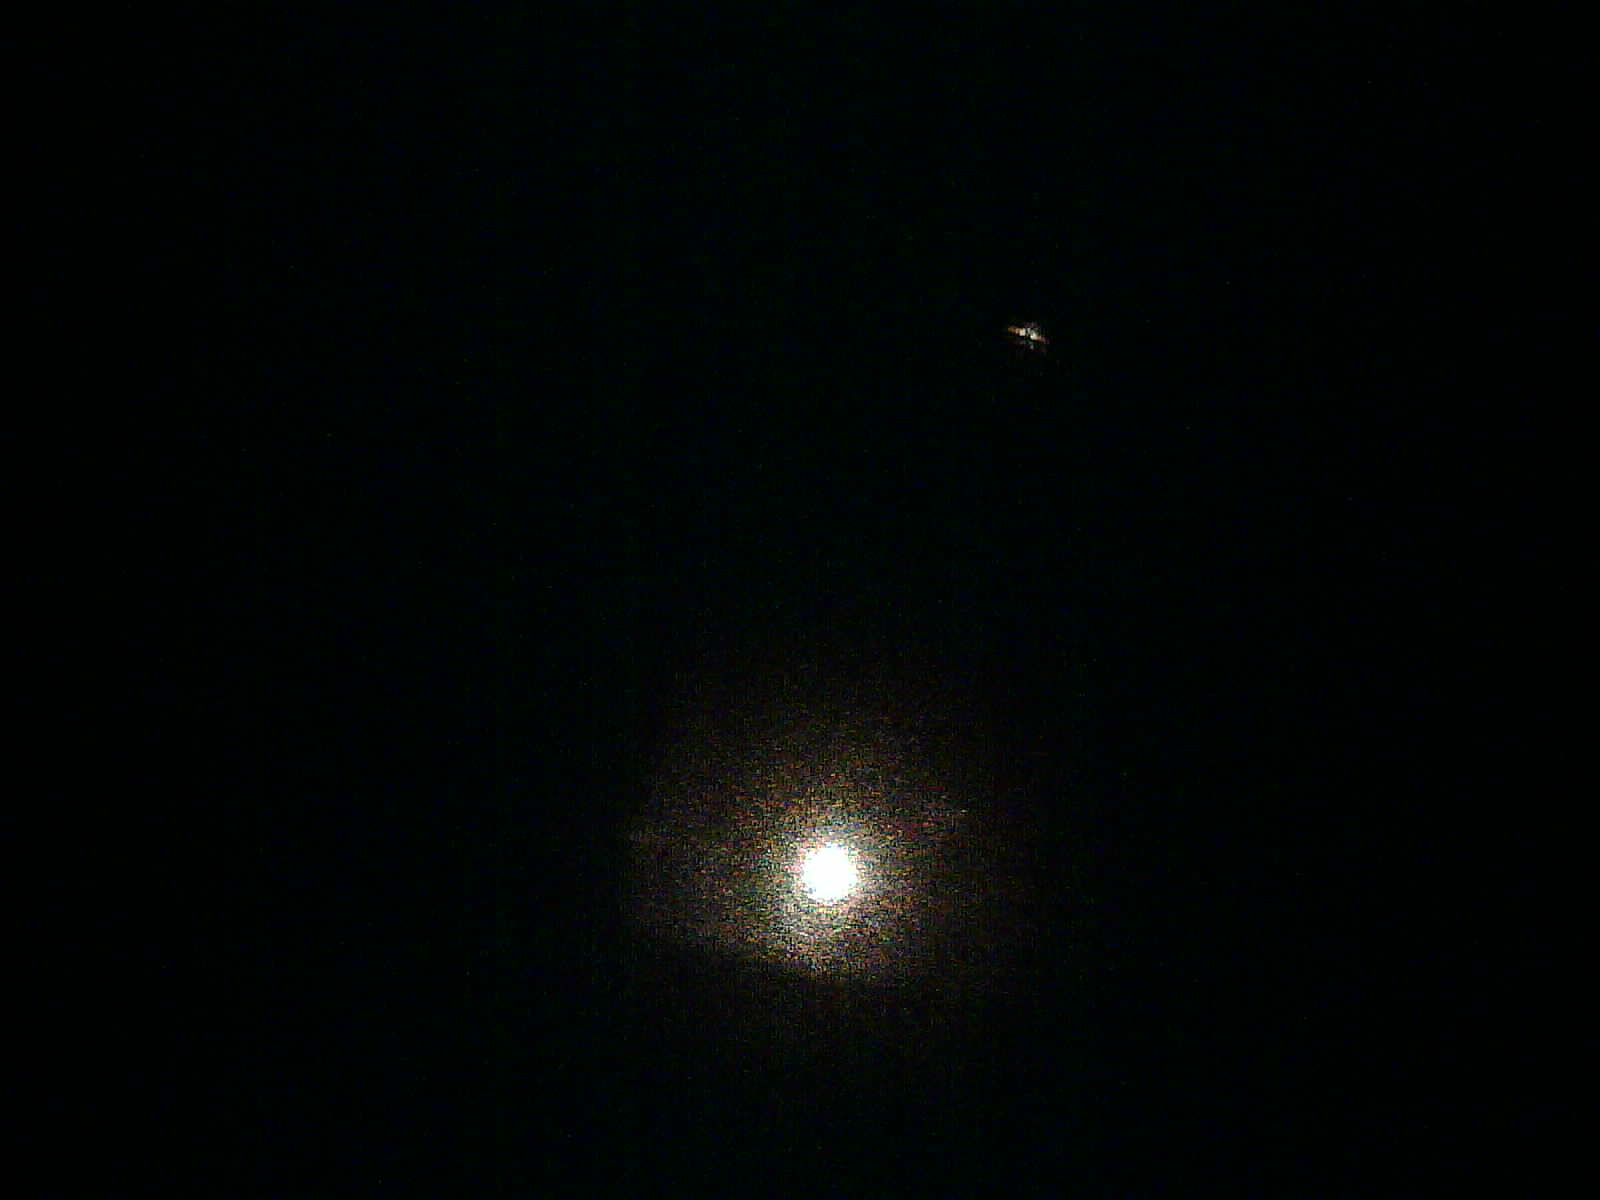
\includegraphics[width=0.5\linewidth]{pics/exposure/5ms}
        \caption{5ms}
        \label{fig:exp5ms}
    \end{subfigure}%
    \begin{subfigure}{0.5\textwidth}
    \centering
        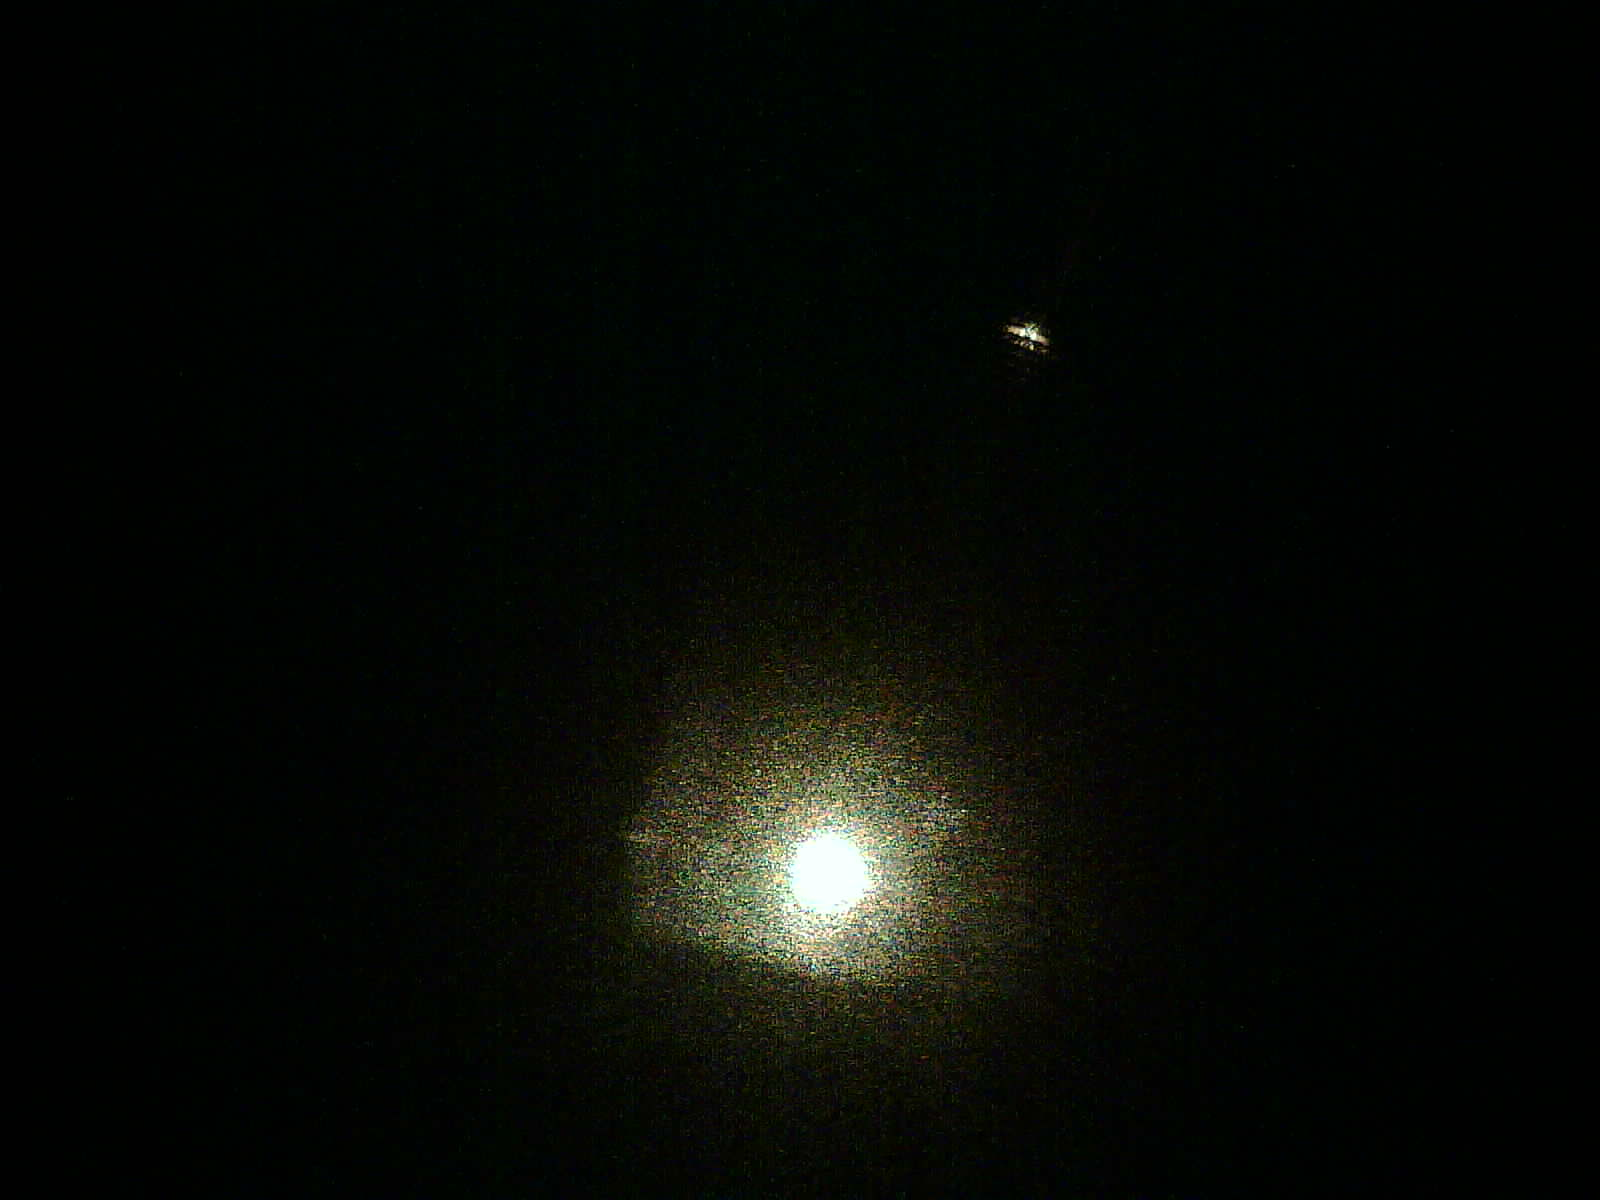
\includegraphics[width=0.5\linewidth]{pics/exposure/10ms}
        \caption{10ms}
        \label{fig:exp10ms}
    \end{subfigure}
        
        \begin{subfigure}{0.5\textwidth}
    \centering
        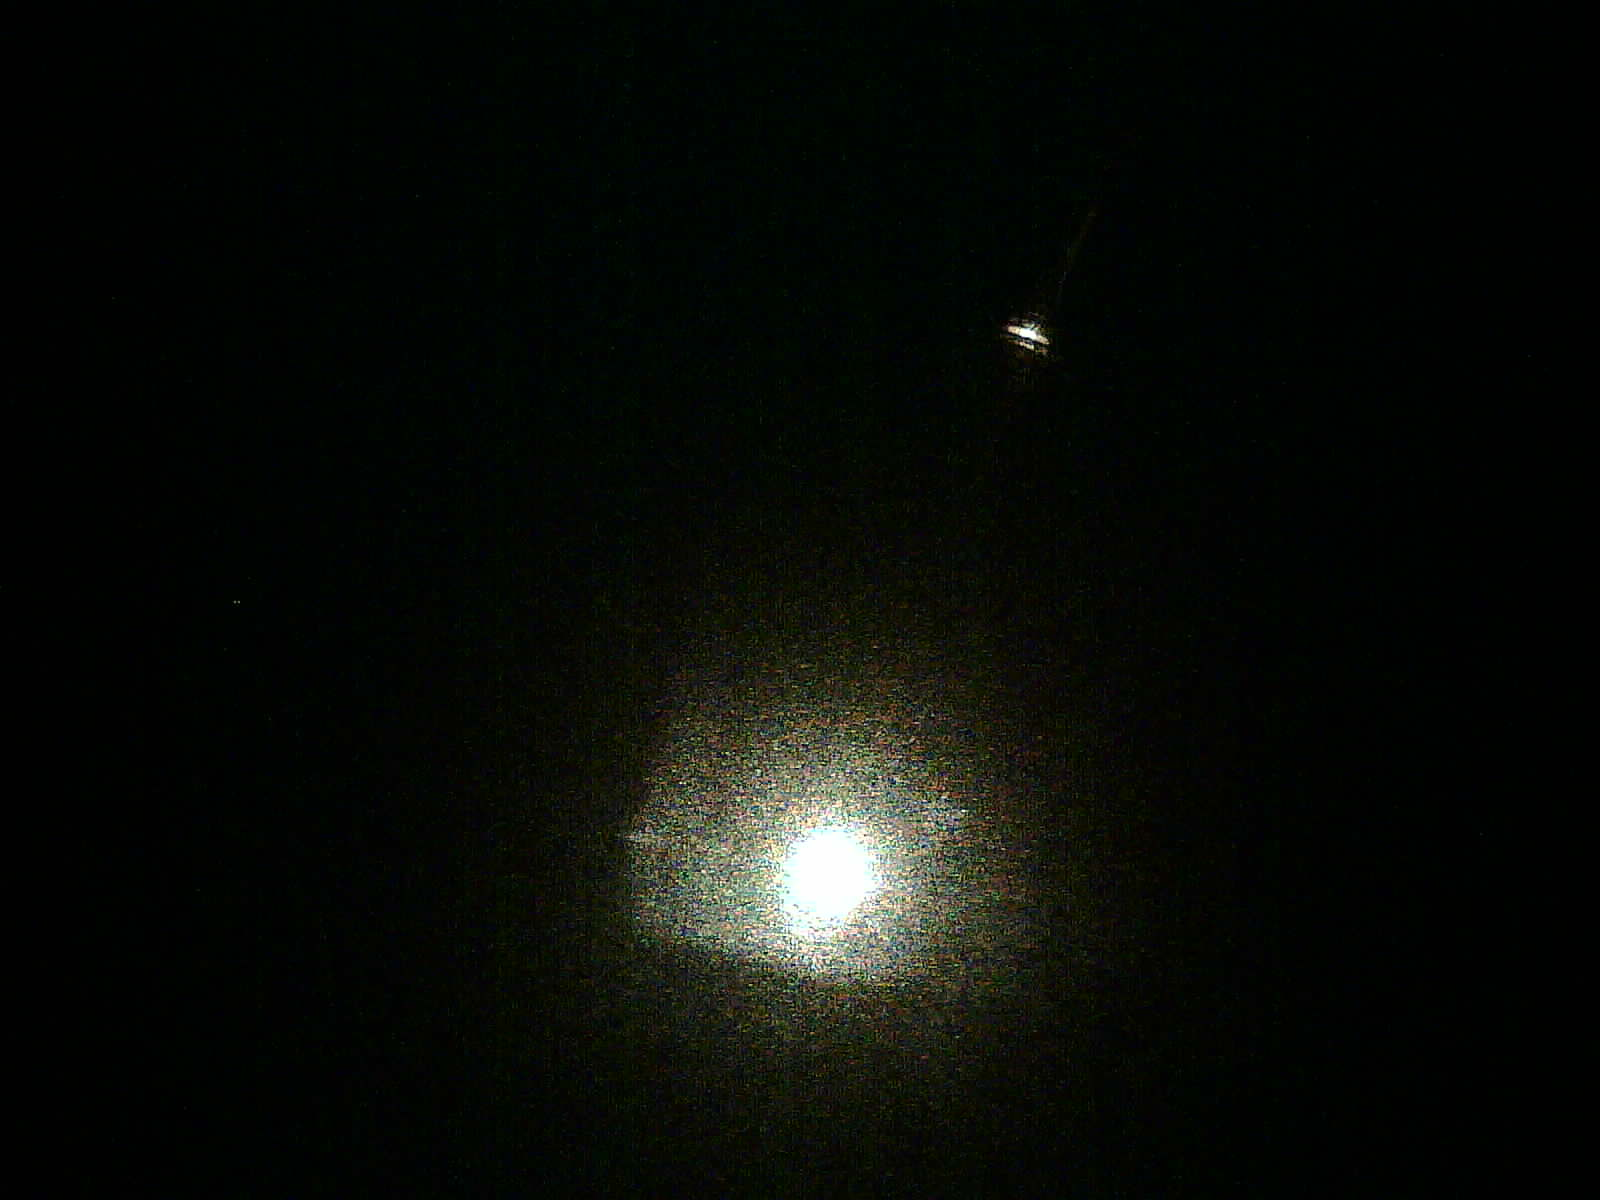
\includegraphics[width=0.5\linewidth]{pics/exposure/20ms}
        \caption{20ms}
        \label{fig:exp20ms}
    \end{subfigure}%
    \begin{subfigure}{0.5\textwidth}
    \centering
        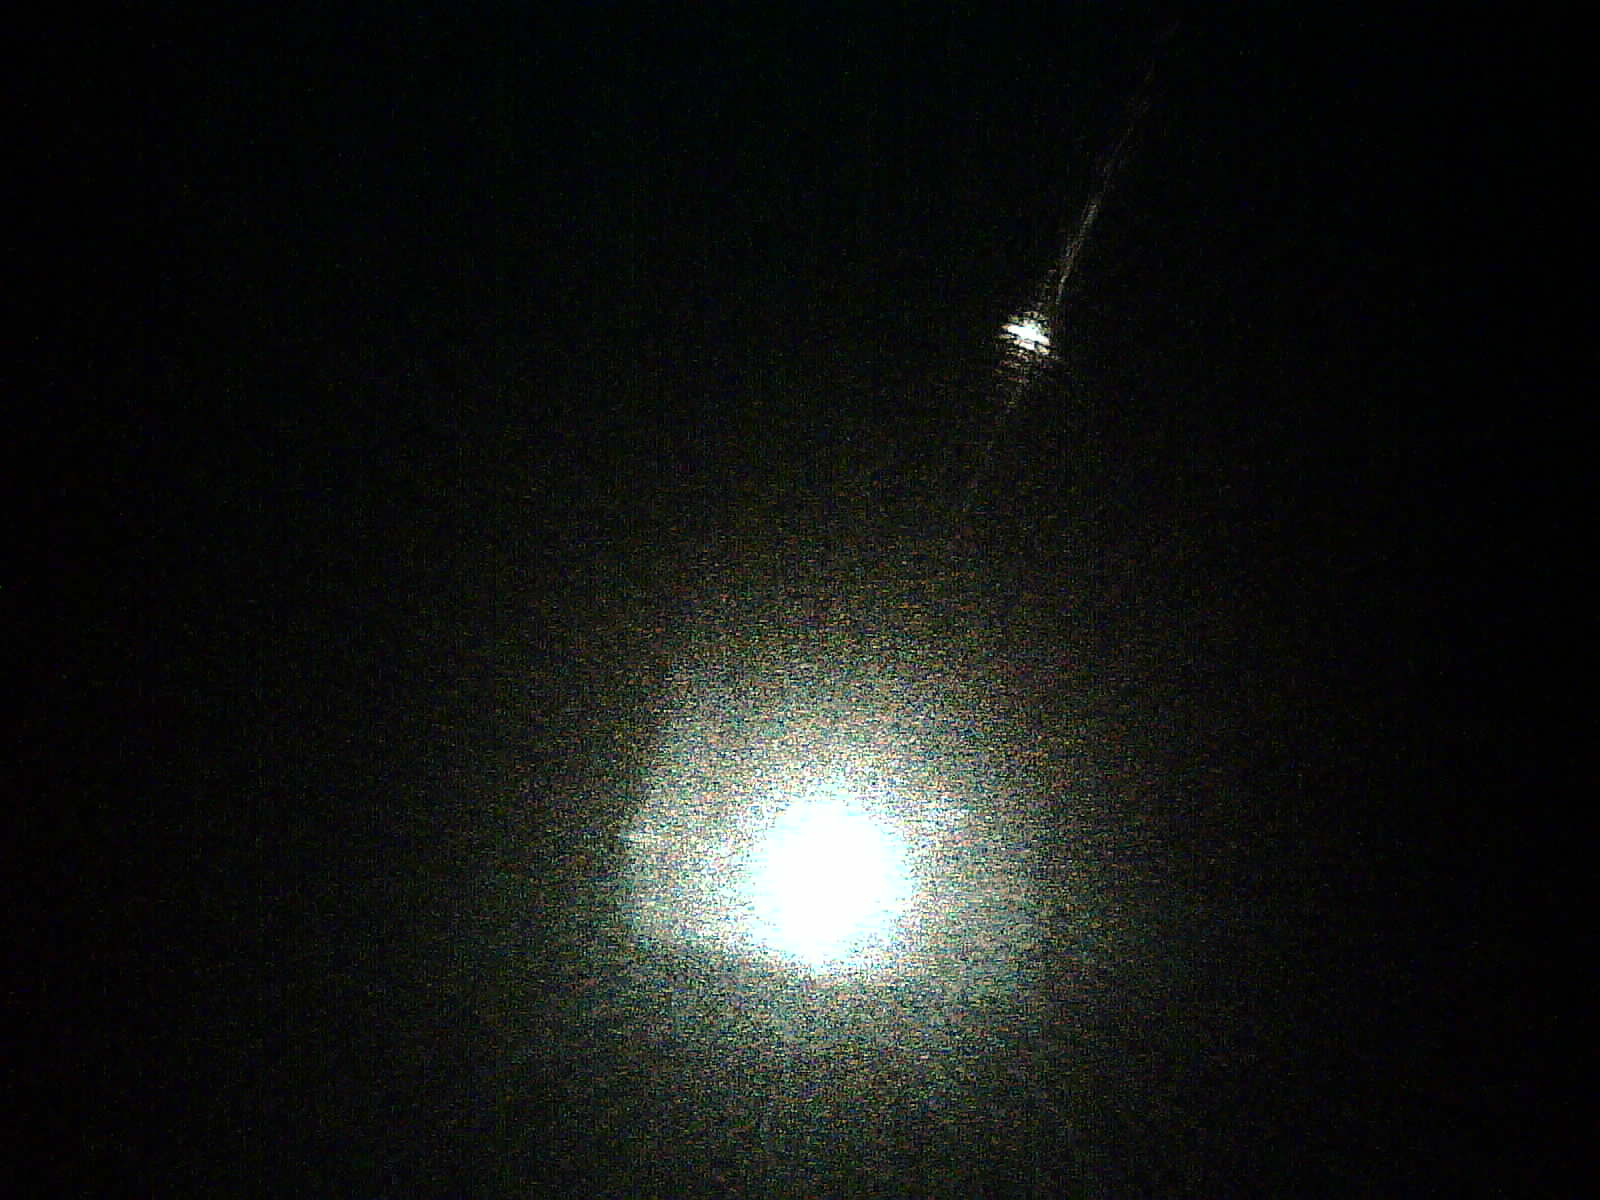
\includegraphics[width=0.5\linewidth]{pics/exposure/60ms}
        \caption{60ms}
        \label{fig:exp60ms}
        
    \end{subfigure}    
    \caption{Images of a laser beam caught in different exposure times(with lens)}
    \label{fig:exptests}
    \end{figure}
    
\section{Power Consumption of Sensors}
 One important aspect that also needs to be taken into account is the power consumption of the camera module(including the sensor, memory, voltage regulators, etc). Since, we have two camera modules, OV2640(low resolution, low power) and OV5642(high resolution, high power). It was decided to perform power consumption measurements for the sensors manually. In order to find the amount of power consumed, we connect a 1 $\Omega$ resistor in series with the power line connecting the microcontroller and CMOS image sensor. The voltage measured across the resistor would be the current consumed by the camera sensors. The camera was operated in two modes: one in continuous ``on" mode and the second mode was ``on only when capture". The second mode was activated clearing \texttt{GPIO\_PWDN\_MASK} when the camera is in use and set it once again once the camera is done taking the pictures and then saving it onto the memory card. This turns off the power supply lines from the Arduino to the when the camera is not taking pictures. The current consumption graph is shown in Figure \ref{fig:power}.
 
   \begin{figure}[ht]
    \centering
    \begin{subfigure}{\textwidth}
    \centering
        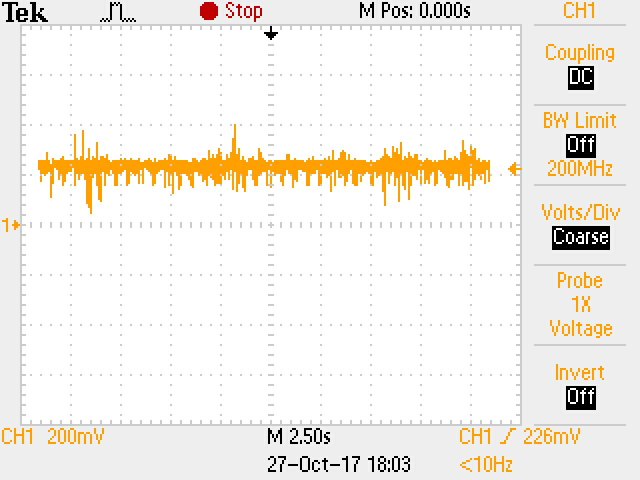
\includegraphics[width=0.75\linewidth]{pics/power_1.JPG}
        \caption{Voltage across  resistor when continuosly on}
    \end{subfigure}%
   
    \begin{subfigure}{\textwidth}
    \centering
        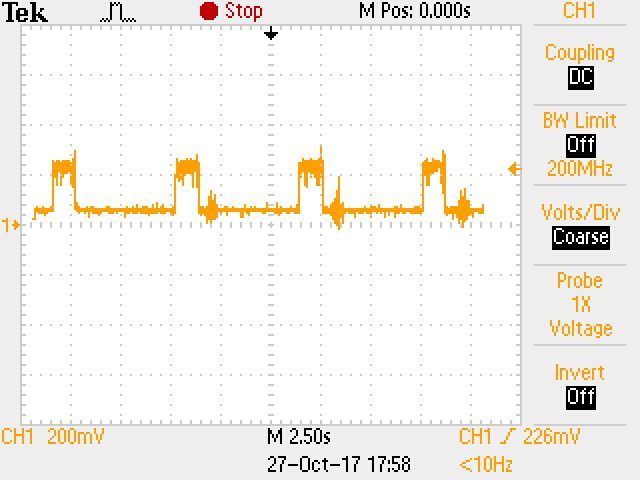
\includegraphics[width=0.75\linewidth]{pics/power_2.JPG}
        \caption{Voltage across  resistor when  using \texttt{GPIO\_PWDN\_MASK}}
    \end{subfigure}
       \caption{This figure shows the difference between keeping the OV5642 sensor module continuously on and using the \texttt{GPIO\_PWDN\_MASK}}
        \label{fig:power}
   \end{figure}

It can be seen from Figure \ref{fig:power} that we can reduce power consumption by switching on the camera only when in use. The camera is operated in 5V mode. The current consumed by the camera is averaged and the measured power consumption is shown in Table \ref{tbl:power_cons}. As expected, the higher resolution camera OV5642 consumes more power than OV2640. Since OV2640 consumes lower power and is also of lower resolution(which implies lesser size of images), we proceed to continue with the next set of experiments using OV2640.
\begin{table}[ht]
\centering
\caption{Measured power consumption of Cameras only when ``on only when capture"}
\label{tbl:power_cons}
\begin{tabular}{|c|c|}
\hline
Sensor & Power \\
\hline
 OV2640 & 5V/93mA\\
 \hline
 OV5642 & 5V/233mA\\
 \hline
\end{tabular}
\end{table}
\nopagebreak
\nolinebreak